\section{Pregunta N$^{\circ}$2\qquad Khalid Zaid Izquierdo Ayllón}

\begin{frame}
	\begin{enumerate}\setcounter{enumi}{1}
		\item

		      Resolver el sistema no lineal
		      \begin{math}
			      \left\{
			      \begin{aligned}
				      x^{2} + y^{2} & = 290 \\
				      x + y         & = 24
			      \end{aligned}
			      \right.
		      \end{math}
		      con los métodos de Newton y
		      homotopía.
	\end{enumerate}

	\begin{solution}
		\begin{figure}[ht!]
			\centering
			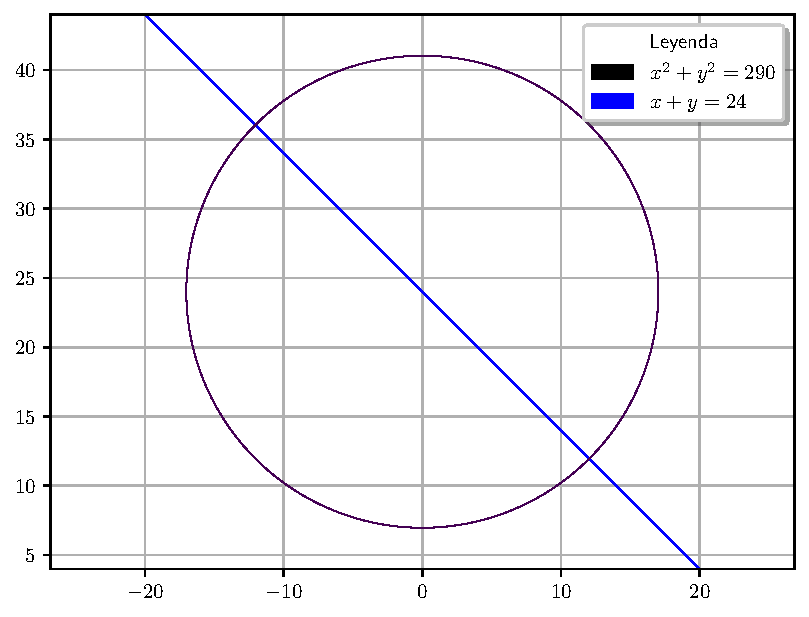
\includegraphics[width=0.5\paperwidth]{p2}
		\end{figure}
	\end{solution}
\end{frame}